\pdfoutput=1 
\documentclass[10pt,conference]{IEEEtran}

\usepackage[T1]{fontenc} % optional
\usepackage{amsmath,amssymb,amsfonts}
%\usepackage[cmintegrals]{newtxmath}
\usepackage{cite}
\usepackage{algorithmic}
\usepackage{graphicx}
\usepackage{textcomp}
\usepackage{xcolor}
\usepackage{multirow}
\usepackage{subcaption}
\usepackage{lipsum}

%\setcitestyle{nocompress}
\usepackage[normalem]{ulem}
%\usepackage[numbers,sort]{natbib}

\usepackage{todonotes}
\usepackage{url}
\usepackage{graphicx}
\usepackage{xspace}
\usepackage{tikz,pgfplots}

\usepgfplotslibrary{statistics}


\newcommand{\system}{\textsc{Groot}\xspace}


\newcommand{\aftertao}[1]{{\color{blue}#1}}

\begin{document}

\title{Groot: An Event-graph-based Approach for Root Cause Analysis in Industrial Settings}

\author{
\IEEEauthorblockN{Hanzhang Wang\IEEEauthorrefmark{1}, Zhengkai Wu\IEEEauthorrefmark{2},
Huai Jiang\IEEEauthorrefmark{1},
Yichao Huang\IEEEauthorrefmark{1},
\\Jiamu Wang\IEEEauthorrefmark{1},
Selcuk Kopru\IEEEauthorrefmark{1},
Tao Xie\IEEEauthorrefmark{4}}
%\vspace{0.05in}
\IEEEauthorblockA{\IEEEauthorrefmark{1}eBay, \IEEEauthorrefmark{2}University of Illinois at Urbana-Champaign, \IEEEauthorrefmark{4}Peking University}

\IEEEauthorblockA{Email: \{hanzwang,huajiang,yichhuang,jiamuwang,skopru\}@ebay.com,
 zw3@illinois.edu,
%\IEEEauthorrefmark{6}huajiang@ebay.com,
%\IEEEauthorrefmark{7}yichhuang@ebay.com,
%\IEEEauthorrefmark{8}\\jiamuwang@ebay.com,
%\IEEEauthorrefmark{9}skopru@ebay.com,
taoxie@pku.edu.cn}
%\vspace{0.05in}
}

\maketitle

\begingroup\renewcommand\thefootnote{\textsection}
\footnotetext{Tao Xie is also affiliated with Key Laboratory of High Confidence Software Technologies (Peking University), Ministry of Education, China. Hanzhang Wang is the corresponding author.}
%Zhengkai Wu's work is supported in part by NSF grant no. CCF-1816615.}
\endgroup
%\thispagestyle{plain}
%\pagestyle{plain}

\begin{abstract}

For large-scale distributed systems, it is crucial to efficiently diagnose the root causes of incidents to maintain high system availability. The recent development of microservice architecture brings three major challenges (i.e., complexities of operation, system scale, and monitoring) to root cause analysis (RCA) in industrial settings. To tackle these challenges, in this paper, we present \system, an event-graph-based approach for RCA. \system constructs a real-time causality graph based on events that summarize various types of metrics, logs, and activities in the system under analysis. Moreover, to incorporate domain knowledge from site reliability engineering (SRE) engineers, \system can be customized with user-defined events and domain-specific rules. Currently, \system supports RCA among \textit{5,000} real production services and is actively used by the SRE teams in eBay, a global e-commerce system serving more than \textit{159 million} active buyers per year. Over 15 months, we collect a data set containing labeled root causes of 952 real production incidents for evaluation. The evaluation results show that \system is able to achieve 95\% top-3 accuracy and 78\% top-1 accuracy. To share our experience in deploying and adopting RCA in industrial settings, we conduct a survey to show that users of \system find it helpful and easy to use. We also share the lessons learned from deploying and adopting \system to solve RCA problems in production environments.

% Groot firstly construct application run-time application dependency graph; then connects "events" such as developer activities, and distributed low-level monitoring events generated by real-time anomaly detection models; and do root cause analysis at the event level on a dynamic event graph.
\end{abstract}

\begin{IEEEkeywords}
microservices, root cause analysis, AIOps, observability
\end{IEEEkeywords}

Reinforcement learning has achieved great success in areas such as Game-playing \citep{silver2018general,vinyals2019grandmaster}, robotics \cite{kober2013reinforcement}, large language models \citep{ouyang2022training}, etc.
However, due to safety concerns or physical limitations, in some real-world reinforcement learning problems, we must consider additional constraints that may influence the optimal policy and the learning process \citep{garcia2015comprehensive}.
% For example, a robotic arm must not take actions that may cause harm to itself or the environments.
A standard framework to handle such cases is the constrained Markov Decision Process (CMDP) \citep{altman1999constrained}.
Within the CMDP framework, the agent has to maximize
the expected cumulative reward while
obeying a finite number of constraints, which are usually in the form of expected cumulative cost criteria.

However, we are sometimes concerned with the problem with a continuum of constraints.
For example,
the constraints we meet might be time-evolving or subject to uncertain parameters, which
cannot be formulated as an ordinary CMDP
(see Examples \ref{Example_Time_Evolving} and  \ref{Example_Uncertain}).
In this paper we would study a generalized CMDP  
to address the above problem.  Because the constraints are not only infinite-number but also lie
in a continuous set,
the generalization is not trivial. Fortunately, we find that we can borrow the idea behind semi-infinite programming (SIP) \citep{remez1934determination, hettich1993semi} to deal with the semi-infinite constraints.
Accordingly, we propose \emph{semi-infinitely constrained Markov decision processes} (SICMDPs)
as a novel complement to the ordinary CMDP framework.
%More specifically,  an SICMDP model %, we consider 
%contains a continuum of constraints whereas an ordinary CMDP contains a finite number of constraints. 

%This generalization is natural but not trivial. However, we can brows the idea  
%The idea is quite natural and can be backtracked
%to the practice of extending linear programming to linear semi-infinite programming (LSIP) %\cite{remez1934determination, GobernaLSIO1998}.
%In addition, 
%As a complementary approach to the ordinary CMDP framework, 
%SICMDP can be used to model these problems  which cannot be described by a finite number of constraints
%that are not covered by .
%For example,
%the restrictions we consider can be time-evolving or subject to uncertain parameters
%, thus
%cannot be described by a finite number of constraints but a continuum of constraints 
%(see Examples \ref{Example_Time_Evolving} and  \ref{Example_Uncertain}).

We also present two reinforcement learning algorithms to solve SICMDPs called SI-CRL and SI-CPO, respectively.
SI-CRL is a model-based reinforcement learning algorithm designed for tabular cases, and SI-CPO is a policy optimization algorithm for non-tabular cases.
% and analyze its performance both theoretically and empirically.
The main challenge is that we need to deal with a continuum of constraints, thus reinforcement learning algorithms for ordinary CMDPs do not work anymore.
In SI-CRL, we tackle this difficulty by first transforming the reinforcement learning problem to an equivalent LSIP problem, which can then be solved using methods in the LSIP literature like the dual exchange methods \citep{Hu1990,reemtsen1998numerical}.
In SI-CPO, we resort to the idea of cooperative stochastic approximation developed in \cite{lan2020algorithms, wei2020comirror}.
As far as we know, we are the first to introduce tools from semi-infinitely programming (SIP) into the reinforcement learning community for solving constrained reinforcement learning problems.

% To the best of our knowledge, we are the first to apply tools from semi-infinitely programming (SIP) to solve reinforcement learning problems.
Furthermore, we give theoretical analysis for both SI-CRL and SI-CPO.
We decompose the error of SI-CRL into two parts: the statistical error from approximating the true SICMDP with an offline dataset and the optimization error due to the fact that the solution of the LSIP problem obtained by the dual exchange method is inexact.
On the optimization side, we show that the iteration complexity of SI-CRL is $O\left(\left\{\mathrm{diam}(Y)L\sqrt{|\gS|^2|\gA|m}/\left[(1-\gamma)\epsilon\right]\right\}^m\right)$.
On the statistical side, we show that the sample complexity of SI-CRL is $\widetilde O\left(\frac{|S|^2|A|^2}{\epsilon^2(1-\gamma)^3}\right)$ if the offline dataset is generated by a generative model, and $\widetilde O\left(\frac{|S||A|}{\nu_{\min} \epsilon^2(1-\gamma)^3}\right)$ if the dataset is generated by a probability measure $\nu$ as considered in \cite{chen2019information}.
Here $\widetilde O$ means that all logarithm terms are discarded.
For SI-CPO, things become a little more complicated because other than the statistical error and the optimization error, we also need to consider the function approximation error, which comes from imperfect policy parametrizations.
It is shown if the function approximation error can be controlled to $O(\epsilon)$ order, the iteration complexity of SI-CPO is $\widetilde{O}\left(\frac{1}{\epsilon^2(1-\gamma)^6}\right)$ and the sample complexity of SI-CPO is $\widetilde{O}(\frac{1}{\epsilon^4(1-\gamma)^{10}})$.
Here our iteration complexity bound is equivalent to a typical $\widetilde O(1/\sqrt{T})$ global convergence rate.

We perform a set of numerical experiments to illustrate the SICMDP model and validate our proposed algorithms.
Specifically, we examine two numerical examples, namely the discharge of sewage and ship route planning.
Through the discharge of sewage example, we show the advantage of the SICMDP framework over the CMDP baseline obtained by naive discretization in modeling realistic sequential decision-making problems.
Moreover, we demonstrate the effectiveness of the SI-CRL and SI-CPO algorithms in such tabular environments. 
In the ship route planning example, we illustrate the benefits of the SICMDP framework and the ability of the SI-CPO algorithm to address complex continuous control tasks involving continuous state spaces with modern deep reinforcement learning techniques.

% In summary, our contributions are listed as follows.
% First, we present the SICMDP model, which can be viewed as a generalization of the ordinary CMDP model.
% Second, we propose an algorithm to perform reinforcement learning for SICMDPs, which is called SI-CRL, and we believe that we are the first to apply tools from SIP
% to solve reinforcement learning problems.
% Third, we give a theoretical analysis of SI-CRL and identify both its sample complexity and iteration complexity.
% In addition, we perform numerical experiments to illustrate the SICMDP model and validate the SI-CRL algorithm.
% \{This paragraph can be removed!!! \}





\textbf{Related work}:
% Object detection related datasets/algo in non-medical domain
% Locally labeled CXR dataset
A few CXR datasets have localized abnormality annotations \cite{shih2019augmenting,filice2020crowdsourcing,jaeger2014two} that are curated manually. These are high quality gold standard ground truth datasets but tend to be smaller in scale (< 30,000 images) and have a narrow coverage, with typically only 1-2 labels. In addition, since most labeling efforts only have abnormality semantics attached, no direct relationships with the affected anatomical locations are available. 

%MEHDI: repeated concepts from above. I am removing the following: 

%The lack of anatomic semantics in the annotation is a limitation for complex multi-modal clinical reasoning work, e.g., differential diagnosis, since clinicians often integrate information along anatomical lines, and for downstream report generation tasks, which often requires describing not only the abnormality but also correctly communicate the location of the abnormalities (and medical devices) to the receiving clinicians. 

Two recent CXR datasets have labels for anatomies described in the reports. In \cite{datta2020dataset}, a small manually annotated dataset (2000 reports) included 10 abnormalities that are individually associated with 29 unique spatial locations (anatomies) at the report level. Another CXR dataset has automatically extracted abnormality and anatomy labels as disconnected concepts that are only correlated at the study level from  160,000 reports using a supervised NLP algorithm \cite{bustos2020padchest}. This was trained on a smaller set of manually annotated data. Neither datasets contain localized annotations for the associated CXR images, nor any comparison relation annotations between sequential exams, both of which are available in the Chest ImaGenome dataset. In Table \ref{tab:related}, we present a comparison of our Chest ImagGenome dataset with other datasets available in the literature.

% Table -- Kashyap

% MEdical imaging datasets to go here: Discussed that we will only focus on cxr datasets that are available for this paper. 
% \caption{\color{red} Kashyap, feel free to continue with the table. We should remove the questionmarks and add a line for our dataset (since all others are not graph). For longer text, using abbreviations and explaining them in the caption often works better. If fill in the values is not possible, it is better to remove the table altogether.}


\begin{table}[t!]
\caption{Summary of existing chest X-ray datasets}
\resizebox{\textwidth}{!}{%
\begin{tabular}{@{}lllllllll@{}}
\toprule
\textbf{Dataset} & \textbf{Annotation Level} & \textbf{Annotation Method} & \textbf{Num Labels} & \textbf{Anatomy Labeled} & \textbf{Graph} & \textbf{Dataset Size} & \textbf{Temporal Labels} & \textbf{Reports} \\ \midrule
SIIM-ACR Pneumothorax Segmentation \cite{filice2020crowdsourcing} & Segmentation & Manual + augmented & 1 & No & No & 12,047 & No & No \\
RSNA Pneumonia Detection Challenge   \cite{shih2019augmenting} & Bounding Boxes & Manual & 1 & No & No & 30,000 & No & No \\
Indiana University Chest X-ray collection \cite{demner2016preparing} & Global & Automated & 10 & No & No & 3,813 & No & Yes \\
NIH CXR dataset \cite{wang2017chestx} & Global & Automated & 14 & No & No & 112,120 & No & No \\
PLCO \cite{team2000prostate} & Global & Automated & 24 & Yes & No & 236,000 & Yes & No \\
Stanford CheXpert \cite{irvin2019chexpert} & Global & Automated & 14 & No & No & 224,316 & No & No \\
MIMIC-CXR \cite{johnson2019mimic} & Global & Automated & 14 & No & No & 377,110 & No & Yes \\
Dutta \cite{datta2020dataset} & Global & Manual & 10 & Yes & Yes & 2,000 & No & Yes \\
PadChest \cite{bustos2020padchest} & Global & Manual + automated & 297 & Yes & No & 160,868 & No & Yes \\
Montgomery County Chest X-ray   \cite{jaeger2014two} & Segmentation & Manual & 1 & Yes & No & 138 & No & No \\
Shenzen Hospital Chest X-ray   \cite{jaeger2014two} & Segmentation & Manual & 1 & Yes & No & 662 & No & No \\  \hline \hline
\textbf{Chest ImaGenome} & Bounding Boxes & Automated & 131 & Yes & Yes & 242,072 & Yes & Yes \\
\bottomrule
\end{tabular}%
}
\label{tab:related}
\vspace{-0.4cm}
\end{table}
% removed (Derived from MIMIC-CXR \cite{johnson2019mimic}) % makes table really small



\section{An example}
\label{sec:6}
\begin{figure}[H]

\includegraphics[scale=.6]{schematic}
\centering
\caption{ A sketch of the example constructed in this section. The manifold decomposes into three pieces, left and right caps and a middle region. The loop drawn on the boundary of the left cap only bounds surfaces of high topological complexity that are at least partly contained in the right cap. This ensures the isoperimetric ratio of that loop is very small.}
\label{fig:example_sketch}
\end{figure}

The aim of this section is to show that the first positive eigenvalue of the 1-form Laplacian can vanish exponentially fast in relation to volume. This contrasts the behaviour of the first positive eigenvalue of the Laplacian on functions.

Our construction is similar to that in \cite{BD}. Essentially, we choose a hyperbolic 3-manifold with totally geodesic boundary and glue it to itself using a particular psuedoAnosov with several useful properties. By \cite{BMNS}, this family has geometry that up to bounded error can be understood in terms of a simple model family. Using this model family, we show that one can find curves with uniformly bounded length whose stable commutator length grows exponentially in the volume. We then use the spectral gap upper bound in Theorem A to conclude the first positive eigenvalue vanishes exponentially fast.

Throughout this section, we need to compare geodesic lengths in different submanifolds of a given manifold $M$. Let $|\cdot|_{X}$ denote the geodesic length of a homotopy class of curves relative endpoints in a manifold $X$ and $\text{length}(\cdot)$ be the length in $M$ of the curve. Similarly, when we compute stable commutator length for the fundamental group of a manifold $X$, which may or may not be a submanifold of $M$, we denote it $\scl_X$.

We will need that for certain curves, $\scl$ is comparable to length. We begin with a simple but essential technical lemma.
\begin{figure}[H]
\labellist
\small\hair 2pt
 \pinlabel {$a_0$} [ ] at 830 1100
 \pinlabel {$a_1$} [ ] at 1300 1100
 \pinlabel {$b_0$} [ ] at 830 1250
 \pinlabel {$b_1$} [ ] at 1300 1250
 \pinlabel {$t_1$} [ ] at 380 1290
 \pinlabel {$t_0$} [ ] at 380 1120
\endlabellist
\centering
\includegraphics[width = 15cm]{lemdiagram}
\caption{ Illustrating Lemma \ref{lem:6.1} , the rectangular base of the figure is part of the totally geodesic surface $S$ and the box is the corresponding part of the tubular neighborhood $N_\e(S)$ foliated by surfaces $S_t$ parallel to $S$. Drawn in the box is the surface $\Sigma$, which is transverse the foliation except at isolated points. The multicurve $a_0\cup a_1$ is part of a single level set $S_{t_0} \cap \Sigma$, but only $a_0$ is part of the curve $c_{t_0}$ described in the lemma, whereas the multicurve $b_0\cup b_1$ forms the multicurve $c_{t_1}$ in the lemma.}
\label{fig:box}
\end{figure}


\begin{lem} \label{lem:6.1} Let $M$ be a compact hyperbolic 3-manifold with totally geodesic boundary $ \d M = S$. Let $\e$ be smaller than the injectivity radius of $M$ and such that $N_\e(S)$ is an embedded tubular neighborhood. Let $\{S_t\}$ be the leaves of the foliation of $N_\e(S)$ by surfaces equidistant from $S$.  Let $\Sigma$ be a smooth incompressible proper not necessarily immersed surface in $M$ that is transverse to the foliation $\{S_t\}$ except at isolated points. Let $c = \d \Sigma$. By transversality, for generic $t$ the multicurve $c_t$ given by the part of $S_t\cap \Sigma$ that cobounds a subsurface of $\Sigma$ with $c = c_0$ is a smooth multicurve.  Let $T$ be the set (of full measure) of all $t\in[0,\e)$ such that $c_t$ is a smooth multicurve. Since $S$ is totally geodesic, each multicurve $c_t$ is homotopic to a possibly degenerate geodesic multicurve $\gamma_t$ in $S$. Let $\Sigma_\e$ be the part of $\Sigma$ contained in $N_\e(S)$. Then for $C = 1/\e$, we have that $$\inf\limits_{t\in T} |\gamma_t|_{S} \leq C \emph{Area}(\Sigma_\e).$$
\end{lem}

\begin{proof} The coarea formula implies the inequality $\inf\limits_{t\in T} |c_t|_{S_t} \leq C \text{Area}(\Sigma_\e)$.  Since $S$ is totally geodesic, for all $t\in T$, we have $|\gamma_t|_S\leq |c_t|_{S_t}.$  \end{proof}
Note that in the previous lemma, when $\inf\limits_{t\in T} |\gamma_t|_S$ is zero, because $\Sigma$ is incompressible and any loop with length less than $\inj(M)$ bounds a disk, every component of $\Sigma$ can either be homotoped to be disjoint from $N_\e(S)$ or be contained in $S$.

The next proposition requires a notion of geometric complexity for homology classes. For any compact Riemannian manifold $M$ one can define the stable norm on the first homology of $M$ (see \cite{Gromovmetric} Section 4C). The mass of a Lipschitz 1-chain $\alpha = \sum_i t_i\alpha_i$ in $M$ is defined to be $\text{mass}(\alpha) = \sum_i |t_i|\text{length}(\alpha_i).$ The mass of a class $a\in H_1(M)$ is then the infimal value of the mass of a chain $\alpha$ representing $a$.
For a class $a\in H_1(M)$, the stable norm of $a$ is then given by $$||a||_{s,M} = \inf\limits_{m>0}\frac{\text{mass}(m a)}{m}.$$

Stable commutator length can also be generalized to geodesic multicurves (see Section 2.6 of \cite{Calegari}), which can naturally be viewed as Lipschitz chains. Suppose $\gamma_i\in \pi_1 M$ and $ \sum_i n [\gamma_i] = 0$ in $H_1(M)$. Let $\gamma$ be the geodesic multicurve, which is not necessarily simple, consisting of the geodesic loops determined by $\gamma_i$. Say a surface $f:S\to M$ is admissible of degree $n(S)$ if it has no closed components and $\d S$ is a union of circles $S^1_i$ with $f|_{S^1_i}$ a degree $n(S)$ cover of $\gamma_i$.
Then we define stable commutator length of $\gamma$ to be $$\scl(\gamma) = \inf\limits_{S \text{ admissible}} \frac{\chi_-(S)}{2n(S)}.$$ When $\gamma$ is a single loop, this definition agrees with the usual definition of stable commutator length.

 \begin{prop} \label{prop:6.2} Let $M$ be a compact oriented hyperbolic 3-manifold with totally geodesic boundary $\d M = S$. Let $\gamma$ be a geodesic multicurve in $S$ that is rationally nullhomologous in $M$. Then there is a constant $D> 0$ depending only on $M$ such that $$||[\gamma]||_{s,S}\leq D\scl_M(\gamma).$$ \end{prop}

 \begin{proof} If $\gamma$ is nullhomologous in $S$, then the left hand side is zero and the inequality holds. Assume now that $[\gamma]\neq 0\in H_1(S)$. Fix $\delta>0$. Let $\Sigma_m$ be an incompressible admissible surface for $\gamma$ of degree $m = n(S)$ such that $\chi_-(\Sigma_m)/2m -\scl(\gamma) < \delta$. We can triangulate $\Sigma_m$ so that there is a single vertex on each boundary component. This triangulation has $4g +3b - 4$ faces, where $g$ is the genus of $\Sigma_m$ and $b$ the number of boundary components. We can then straighten this triangulation to obtain a piecewise totally geodesic triangulated surface. Replace $\Sigma_m$ with this surface. Since every face of this triangulation of $\Sigma_m$ is geodesic, every face has area at most $\pi$. Since there are $4g+3b - 4$ faces and $\chi_-(\Sigma_m) = 2g-2 + b$, we can estimate  $$\text{Area}(\Sigma_m) \leq 3\pi\chi_-(\Sigma_m).$$

We can perturb $\Sigma_m$ to obtain a smooth surface $\Sigma’_m$ that it is transverse the foliation of $N_\e(S)$ except at isolated points and in doing so increase the area by less than $\delta$. Let $\gamma_t$ be the family of multicurves in Lemma \ref{lem:6.1}  applied to $\Sigma’_m$. Since each curve $\gamma_t$ cobounds a surface in $S$ with $\d \Sigma_m$, they are homologous, thus $||[\gamma_t]||_{s,S} = m||[\gamma]||_{s,S}$. Since $||[\gamma_t]||_{s,S}\leq |\gamma_t|_S$,
Lemma \ref{lem:6.1}  implies that $$m||[\gamma]||_{s,S}\leq C\text{Area}(\Sigma_m’) \leq C \text{Area}(\Sigma_m) + C\delta \leq 3C\pi\chi_-(\Sigma_m) + C\delta.$$
From this we get  $$||[\gamma]||_{s,S}\leq 6C\pi\chi_-(\Sigma_m)/2m + C\delta/m\leq 6C\pi\scl_M(\gamma) + 6C\pi\delta +C\delta/m.$$
Since the stable commutator length of a nontrivial rational commutator is bounded away from zero by a constant only depending on $M$, by Theorem 3.9 in \cite{Calegari}, we can replace $C$ with a larger constant $D$ such that $$||[\gamma]||_{s,S}\leq D\scl_M(\gamma),$$ as desired. \end{proof}

 We now introduce the family of manifolds that we use in our construction. The family $\{W_n\}$ of manifolds we study are easily understood using the model manifold theory of \cite{BMNS}. In particular, there is a $K$-biLipschitz map between $W_n$ and a model manifold $M_n$, where $K$ is independent of $n$. The base of the construction is Thurston’s tripus manifold $W$ (see \cite{thurstonbook}, Section 3.3.12), a hyperbolic manifold with totally geodesic boundary, and a psuedoAnosov homeomorphism $f$ of the boundary surface $\d W$. The model manifold $ M_n$ is a degree $n$ cyclic cover of the mapping torus $M_{f}$ cut open along a fiber with two oppositely oriented copies of $W$, denoted $W^+$ and $W^-$ glued as described in \cite{BMNS} Section 2.15 to the two boundary components of the cut open mapping torus. This decomposes $W_n$ into three pieces, a product region $S\times [0, n]$ and the caps $W^+$ and $W^-$ in a metrically controlled way. It will be convenient to set $M^+ = W^+\subset M_n$ and $M^- = W^-\subset M_n$ when talking about the caps of the model manifold $M_n$ for fixed $n$, and to let $W^+$ and $W^-$ denote the images of these spaces under the natural inclusion into $W_n$.

 \vspace{1cm}
\begin{figure}[H]
\labellist
\small\hair 2pt
 \pinlabel {$M^+$} [ ] at 950 1100
 \pinlabel {$M^-$} [ ] at 2000 1100
 \pinlabel {$S\times[0,n]$} [ ] at 1500 1600
\endlabellist
\centering
\includegraphics[scale=.15]{modelscheme}
\caption{ A schematic picture of the model manifold $M_n$ with caps $M^+$ and $M^-$ two oppositely oriented copies of the tripus manifold.}
\label{fig:caps_schematic}
\end{figure}

Given a multicurve $c$ in $M^{\pm}$, we say $c$ \textbf{bounds on both sides} if there are incompressible surfaces $S^+$ in $M^+$ and $S^-$ in $M^-$ both with boundary homotopic to $c$.

We encode the construction and its essential properties in the following proposition.

\begin{prop}  \label{prop:6.3}There is a family $\{W_n\}$ of closed hyperbolic 3-manifolds with injectivity radius uniformly bounded below and volume growing linearly in $n$ constructed from the tripus and a pseudoAnosov $f$ as described above. Each manifold $W_n$ is $K$-biLipschitz equivalent to the model manifold $M_n$ for some constant $K$ independent of $n$. Any homologically nontrivial loop in $H_1(\d W^{\pm})$ that bounds a surface in $M^{\pm}$ cannot bound on both sides. The pseudoAnosov $f$ is such that for any nonzero class $a\in H_1(\d W^+)$, the stable norm of $f_*^n(a)$ grows exponentially.
\end{prop}

\begin{proof}
Let $W$ be Thurston’s tripus manifold, a compact hyperbolic 3-manifold with totally geodesic boundary a genus 2 surface for which the inclusion map $H_1(\d W;\Z)\to H_1(W;\Z)$ is onto.
The homology of the boundary $\d W$ decomposes as the direct sum of rank 2 submodules $U$ and $V$, where $V\subset H_1(\d W)$ is the image of the boundary map $\d : H_2(W,\d W;\Z)\to H_1(\d W;\Z)$ (which is also the kernel of the inclusion $H_1(\d W)\to H_1(W)$) and $U$ is a compliment of $V$ (note that the inclusion map $H_1(\d W)\to H_1(W)$ restricted to $U$ is an isomorphism).
Let $S$ be a genus 2 surface, which we will use to mark the boundaries of $W^{+}$ and $W^-$. Assume $H_1(S;\Z)$ is generated by $e_1,~e_2,~e_3,~e_4$. Choose a marking $S\to \d W^+$ so in $W^+$ one has $U = \langle e_1,e_2\rangle $ and $V = \langle e_3, e_4\rangle$.
Similarly, choose a marking $S\to \d W^-$ so that in $W^-$ one has $V = \langle e_1,e_2\rangle $ and $U = \langle e_3, e_4\rangle$. We then define $$W_n = W^+\cup_{f^n}W^-$$ where $f:S\to S$ is a pseudo-Anosov that acts on $H_1(S)$ by the symplectic matrix\[ F = \begin{pmatrix}
 2 &  1 & 0 & 0 \\
 1 & 1 & 0 & 0 \\
 0 & 0 & 1 & -1\\
 0 & 0 & -1 & 2
\end{pmatrix} \] For the existence of such a pseudoAnosov mapping class, see the proof Lemma 7.1 in \cite{BD}. This matrix preserves the subspace decomposition above, and so ensures that every curve in $\d W^{\pm}$ that is not nullhomologous in $\d W^{\pm}$ but bounds a surface in $M^{\pm}$ cannot bound on both sides.

The mapping class $f$ acts as an Anosov matrix on $U$ and $V$. This ensures the standard Euclidean $\ell^2$-norm $||F^n(a)||_E$ of an element $a\in H_1(S)$ grows exponentially in $n$ (indeed, for our choice of $F$, it grows like $(\frac{3+\sqrt{5}}{2})^n$). Since norms on finite dimensional real vector spaces are comparable, there is a constant comparing the stable norm induced by the metric inherited from $W$ to the standard Euclidean $\ell^2$-norm on $H_1(S)$.

Lemma 7.3 in \cite{BD} explains how Theorem 8.1 in \cite{BMNS} implies that for large $n$ the manifolds $W_n$ admit a $K$-biLipschitz diffeomorphism $\mu$ from the model manifold $ M_n$ as described above. After increasing $K$, we can drop the large $n$ condition. This then also implies the linear volume growth and injectivity radius bounds.
\end{proof}

\begin{remark}
Using the model manifold, one can easily estimate the Cheeger constant of $W_n$, which will decay like $1/n$.
\end{remark}


\begin{mainthm}  \label{thm:C} The family $W_n$ of closed hyperbolic 3-manifolds from Proposition \ref{prop:6.3}  has 1-form Laplacian spectral gap that vanishes exponentially fast in relation to volume:
$$\sqrt{\lambda(W_n)}\leq B\vol(W_n)e^{-r\vol(W_n)},$$
where $r$ and $B$ are positive positive constants and $\lambda(W_n)$ is the first positive eigenvalue of the 1-form Laplacian on $W_n$.
\end{mainthm}


\begin{proof}
We continue using notation introduced in the previous propositions. Take $\gamma$ in $\d M^+\subset M_n$ to be an embedded geodesic loop representing the class $e_1 \in U \subset H_1(\d W^+)$. Recall from the proof of Proposition \ref{prop:6.3} that $\gamma\subset \d M^+$ does not bound a surface in $M^+$ but that $f^n(\gamma)\subset \d M^-$ bounds a surface in $M^-$. Let $\alpha_n = f^n(\gamma)\subset \d M^- \subset M_n$. Note that $\alpha_n$ and $\gamma$ are isotopic in $M_n$.

Fix $\delta>0$. Consider some positive integer $m$ and  incompressible surface $\Sigma_m$ bounding $\alpha_n^m$ in $M_n$ with $\chi_-(\Sigma_m)/2m - \scl_{M_n}(\gamma) < \delta$ and which minimizes $\chi_-$ among surfaces with boundary $\alpha_n^m$. We can then replace $\Sigma_m$ with a homotopic surface that pushes the boundary of $\Sigma_m$ into the interior of $M^-$ and which intersects $\d M^-$ transversely and essentially in both $\d M^-$ and $\Sigma_m$.
We can then attach an annulus to $\Sigma_m$ cobounding $\alpha_n^m$ and the boundary of the modified surface $\Sigma_m$. This new $\Sigma_m$ bounds $\alpha_n^m$ with a collar neighborhood of the boundary contained entirely in $M^-$ and intersects $\d M^-$ transversely in a union of loops essential in both $\Sigma_m$ and $\d M^-$.

We focus on the portion of $\Sigma_m$ that lies in $M^-$. Define $\Sigma^-_m =\Sigma_m\cap M^-$. If $\Sigma_m$ is contained in $M^-$, then Proposition \ref{prop:6.2}  applied to $\alpha_n^m$ in $M^-$ implies that
$$||[\alpha_n^m]||_{s,\d M^-} = m||[\alpha_n]||_{s,\d M^-} \leq m\scl_{M^-}(\alpha_n)\leq D\chi_-(\Sigma_m^-) = D\chi_-(\Sigma_m) ,$$
where $||\cdot||_{s, \d M^-}$ is the stable norm of $H_1(\d M^-)$. Since $\chi_-(\Sigma_m)/m- \scl_{M_n}(\gamma)\leq \delta$, we conclude $$||[\alpha_n]||_{s,\d M^-}\leq D\scl_{M_n}(\gamma) + D\delta.$$

Our goal now is to get this same estimate for the other possible ways $\Sigma_m$ sits in $M_n$.
\vspace{1cm}
\begin{figure}[H]
\labellist
\small\hair 2pt
 \pinlabel {$M^+$} [ ] at 900 1560
 \pinlabel {$S\times[0,n]$} [ ] at 1480 1650
 \pinlabel {$M^-$} [ ] at 2000 1560
 \pinlabel {$\alpha$} [ ] at 1750 1050
\endlabellist
\centering
\includegraphics[scale=.2]{schematic5}
\caption{ A schematic picture of the simplest case of a surface bounding $\alpha$ in $M^-$.}
\label{fig:alpha_bounds}
\end{figure}

Consider the case that $\Sigma_m$ does not lie entirely in $M^-$. There are two possibilities. The first involves the surface $\Sigma_m$ passing into the product region but not intersecting $M^+$. In this case the surface can be homotoped to lie in $M^-$, so that Proposition \ref{prop:6.2} applies, giving the desired estimate as in the previous case.
\vspace{2cm}
\begin{figure}[H]
\labellist
\small\hair 2pt
 \pinlabel {$M^+$} [ ] at 900 1560
 \pinlabel {$S\times[0,n]$} [ ] at 1480 1650
 \pinlabel {$M^-$} [ ] at 2000 1560
 \pinlabel {$\alpha$} [ ] at 1750 850
\endlabellist
\centering

\includegraphics[scale=.2]{schematic3}
\caption{ A schematic picture of a surface bounding $\alpha$ that passes back into $M^-$ but does not pass into $M^+$.}
\label{fig:pass_back_schematic}
\end{figure}

\vspace{2cm}
\begin{figure}[H]
\labellist
\small\hair 2pt
 \pinlabel {$M^+$} [ ] at 900 1560
 \pinlabel {$S\times[0,n]$} [ ] at 1480 1650
 \pinlabel {$M^-$} [ ] at 2000 1560
 \pinlabel {$\alpha$} [ ] at 1750 850
 \pinlabel {$c_1$} [ ] at 1750 1285
 \pinlabel {$c_0$} [ ] at 1750 1070

\endlabellist
\centering

\includegraphics[scale=.2]{schematic6}
\caption{ A schematic picture of a surface bounding $\alpha$ that passes back into $M^+$. Notice the multicurve $c^- = c_0\cup c_1$ bounds surfaces in $M^+$ and $M^-$, so is homologically trivial. }
\label{fig:bounds_both_sides}
\end{figure}



The second possibility concerns the surface $\Sigma_m$ crossing through the product region into $M^+$ with an essential intersection with $\d \Sigma^+$. In this case, we will see that the surface $\Sigma_m^-$ has boundary homologous to $\alpha_n^m$, which will allow us to apply Proposition \ref{prop:6.2} to obtain the desired estimate. By construction, a sufficiently small collar $C$ of the boundary $\d \Sigma_m$ in $\Sigma_m$ maps into $M^-$, so in particular, a subsurface of $\Sigma_m^-$ has some boundary component that maps to $\alpha_n^m$. That boundary component can be closed by attaching a surface $S^-$ that bounds $\alpha_n^m$ in $M^-$ to $\Sigma_m$.
From this, we see that the multicurve $c^- = \d \Sigma^-_m -\alpha_n $ bounds surfaces in $M^+$ and $M^-$.
Thus by Proposition \ref{prop:6.3}, $c^-$ must be homologically trivial in $\d M^{-}$. Let $x = \d\Sigma_m^- = c^- + \alpha_n^m$. Since $c^-$ is nullhomologous, $||[x]||_{s,\d M^-} = ||[\alpha_n^m]||_{s,\d M^-} = m||[\alpha_n]||_{s,\d M^-}.$
By Proposition \ref{prop:6.2} , $||[x]||_{s,\d M^-}\leq D\scl_{M^-}(x).$ Since $x$ is essential in $\Sigma_m$, we get that $\chi_-(\Sigma_m^-) \leq \chi_-(\Sigma_m)$, then using that $\chi_-(\Sigma_m)/2m - \delta \leq \scl_{M_n}(\alpha_n)$,
we obtain $\scl_{M^-}(x) \leq \chi_-(\Sigma_m^-)/2 \leq m\scl_{M_n}(\alpha_n) + \delta m$.
Putting this all together and dividing by $m$, we get that $$||[\alpha_n]||_{s,\d M^-}\leq D\scl_{M_n}(\alpha_n) + D\delta.$$

We therefore have in each case that there is a constant $D$ independent of $n$ such that $$||[\alpha_n]||_{s,\d M^-}\leq D\scl_{M_n}(\alpha_n) + D\delta.$$ By Proposition \ref{prop:6.3} , $||[\alpha_n]||_{s,\d M^-} = ||[f^n(\gamma)]||_{s,\d M^+}$ grows exponentially in $n$.
Thus for some constants $B>0$ and $r >0$, we have $$Be^{rn}\leq D\scl_{M_n}(\gamma) + D\delta,$$ where we use that $\gamma$ and $\alpha_n$ are homotopic in $M_n$. Using the injectivity radius lower bound and Theorem 3.9 of \cite{Calegari}, we can increase $D$ and drop the additive constant in this inequality. By Proposition \ref{prop:6.3} , the volume growth of the $W_n$ is proportional to $n$ so there is a constant $C$ such that $\vol(W_n)\leq Cn$.
Additionally, using the $K$-biLipschitz comparison of Proposition \ref{prop:6.3} , the length of $\gamma$ in $W_n$ is bounded from above by $2K|\gamma|_{W}$, where $W$ is the tripus. As a result, Theorem A implies that the spectral gap for the 1-form Laplacian of the manifolds $W_n$ vanishes exponentially fast in $n$.
In particular, we have \[\sqrt{\lambda(W_n)} \leq A\vol(W_n)\frac{|\gamma|_{W_n}}{\scl_{W_n}(\gamma)} \leq 2KACB^{-1}D|\gamma|_Wne^{-rn},\] so the result holds after redefining $B$ to be $2KACB^{-1}D|\gamma|_W.$

\end{proof}

\section{Approach}
\begin{figure}[t]
\centering
\resizebox{0.48\textwidth}{!}{ 
  \includegraphics[width=\textwidth]{figures/workflow.PNG}
}
  \caption{Workflow of \system}
  \label{fig:workflow}
\end{figure}

Figure ~\ref{fig:workflow} shows the overall workflow of \system. The triggers for using \system are usually alert(s) from automated anomaly detection, or sometimes an SRE engineer's suspicion. There are three major steps: constructing the service  dependency graph, constructing the event causality graph,  and root cause ranking. The outputs are the root causes ranked by the likelihood. To support fast human investigation experience, we build an interactive UI as shown in  Figure~\ref{fig:UI}: the service dependency, events with causal links and additional details such as raw metrics or the developer contact (of a code deployment event) are presented to the user for next steps. As an  offline part of human investigation, we label/collect a data set, perform validation, and summarize the knowledge for further improvement on all incidents on a daily basis. %as validations and heterogeneous graph learning (HGL)~\cite{qiao2020heterogeneous} to synthesize the knowledge from existing cases in order to further improve the system.

\subsection{Constructing Service Dependency Graph}
\label{sec:appgraph}

The construction of the service dependency graph starts with the initial alerted or suspicious service(s), denoted as $I$. For example, in Figure ~\ref{fig:ex1_dep}, $I=\{\textit{Checkout}\}$. $I$ can contain multiple services based on the range of the trigger alerts or suspicions. We maintain domain service lists where domain-level alerts can be triggered because there is no clear service-level indication.

At the back end, \system maintains a global service dependency graph $G_{global}$ via distributed tracing and log analysis. The directed edge from nodes $A$ to $B$ (two services or system components) in the dependency graph indicates a service invocation or other forms of dependency. In Figure~\ref{fig:ex1_dep}, the black arrows indicate such edges. Bi-directional edges and cycles between the services can be possible and exist. In this work, the global dependency graph is updated daily.%by extracting from one day's total site traffic.

The service dependency (sub)graph $G$ is constructed using $G_{global}$ and $I$. An extended service list $L$ is first constructed by traversing each service in $I$ over $G_{global}$ for a radius range $r$. Each service $u \in L$ can be traversed by at least one service $v \in I$ within $r$ steps: $L=\{u|\exists v\in I, \ dist(u,v)\le r\ or\ dist(v,u)\le r\}$. Then, the service dependency subgraph $G$ is constructed by the nodes in $L$ and the edges between them in $G_{global}$. In our current implementation, $r$ is set to $2$, since this dependency graph may be dynamically extended in the next steps based on events' detail for longer issue chains or additional dependencies.

\subsection{Constructing Event Causality Graph}
\label{sec:causality}

In the second step, \system collects all supported events for each service in $G$ and constructs the causal links between events. 

\subsubsection{Collecting Events}

Table~\ref{tab:events} presents some example event types and detection techniques for \system's production implementation. For detection techniques, ``De Facto'' indicates that the event can be directly collected via a specific API or storage. %The detection can be done passively at the back end continuously then store anomaly events in different databases; or done actively by pulling data and run detection on the fly to save compute resources. 
The detection either runs passively in the back end to reduce delay and improve accuracy, or runs actively for only the services within the dependency graph range to save resources. %For example, low-level error signals or logs are detected actively since they are too many to scale. 

There are three major categories of events: performance metrics, status logs, and developer activities:
\begin{itemize}
    \item \emph{Performance metrics} represent an anomaly of monitored time series metrics. For example, high CPU usage indicates that the service is causing high CPU usage on a certain machine. In this category, most events are continuously and passively detected and stored. %For high CPU usage, threshold indicates the event is created when CPU usage is higher than certain predefined value. TPS spike indicates a spike in transaction per second, since TPS is a moving average value, we use some statistical model learned from historical data to detect such events.
    \item \emph{Status logs} are caused by abnormal system status, such as spike of HTTP error code metrics while accessing other services' endpoints. Different types of error metrics are important and supported in \system, including third-party APIs. For example, Bad Host indicates abnormal patterns on some machines running the service, and can be detected by a  clustering-based ML approach.%Markdown indicates that the whole service is down. 
    \item \emph{Developer activities} are the events generated when a certain activity of developers is triggered, such as code deployment and config change.
\end{itemize}

\begin{table}[t]
\centering
\caption{List of example event types used in \system}
\resizebox{0.4\textwidth}{!}{ 
\begin{tabular}{|c|c|c|}
\hline
Type                                & Event Type                  & Detection Technique  \\ \hline
\multirow{6}{*}{Performance Metrics} & High GC (Overhead)      & Rule-based        \\ \cline{2-3} 
                                    & High CPU Usage          & Rule-based        \\ \cline{2-3} 
%                                    & Out of Memory           & Rule-based        \\ \cline{2-3} 
%                                    & LB Connection Stacking  & Statistical Model \\ \cline{2-3} 
                                    & Latency Spike           & Statistical Model \\ \cline{2-3} 
                                    & TPS Spike               & Statistical Model \\ \cline{2-3} 
                                    & Database Anomaly        & ML Model          \\ \cline{2-3} 
                                    & Business Metric Anomaly & ML Model          \\ \hline
\multirow{4}{*}{Status Logs}        & WebAPI Error            & Statistical Model \\ \cline{2-3} 
                                    & Internal Error          & Statistical Model \\ \cline{2-3} 
                                    & ServiceClient Error     & Statistical Model \\ \cline{2-3} 
                                    & Bad Host                & ML Model          \\ \hline %\cline{2-3} 
%                                    & Hystrix Circuit Break   & De Facto          \\ \hline
\multirow{3}{*}{Developer Activities} & Code Deployment         & De Facto          \\ \cline{2-3} 
                                    & Configuration Change    & De Facto          \\ \cline{2-3} 
                                    & Execute URL             & De Facto          \\ \hline
\end{tabular}
}
\label{tab:events}
\end{table}

In Groot, there are more than a dozen event types such as \emph{Latency Spike} as listed in the column 2 of Table~\ref{tab:events}. 
Each event type is characterized by three aspects: $Name$ indicates the name of this event type; $Lookback Period$ %\footnote{In Figure~\ref{fig:ex2_n1}, there are two periods, 1 day indicates the look-back range if the model has already finished deployment, 4 days indicates the range if the model deployment is still ongoing(incremental deployment).} 
indicates the time range to look back (from the time when the use of \system is triggered) for collecting events of this event type;  $PropertyType$ indicates the types of the properties that an event of this event type should hold. 
$PropertType$  is characterized by a vector of pairs, each of which indicates the string type for a property's name and the primitive type for the property's value such as string, integer, and float. 
Formally, an event type is defined as a tuple: 
$ET = <Name, Lookback Period, PropertyType>$ 
where 
$PropertyType = <(string, \textit{type}_1), ..., (string, \textit{type}_{n})>$ ($n$ is the number of properties that an event of this event type holds). 
%

Each event of a certain event type $ET$ is characterized by four aspects:
$\textit{Service}$ indicates the service name that the event belongs to; $\textit{Type}$ indicates $ET$'s $\textit{Name}$;  $\textit{StartTime}$ indicates the time when the event happens; $\textit{Properties}$ indicates the properties that the event  holds.
Formally, an event is defined as a tuple: 
$e = <Service, Type, StartTime, Properties>$ 
where $Properties$ is an instantiation of $ET$'s  $PropertyType$. 


%and each event is defined as $e = \{<\textit{Property}_i, \textit{value}_i>\}$. Each event type serves as a template for the event instantiation. such as a string, an integer, a float or a set of primitive types while $\textit{value}$ is limited to primitive data types. 
%
%Each event is defined as a sequence of property-value pairs where the set size is $n$.

For example, in Figure~\ref{fig:example1}, the generated event for \emph{Latency Spike in DataCenter-A} in \emph{Service-C} would be $<``\textit{Service-C}'', ``\textit{Latency\ Spike}'', \textit{2021/08/01-12:36:04}, <(``\textit{DataCenter}'',``\textit{DC-1}''),  ...>>$. %So for each service in $G$, we detect/collect and filter the events within specified time range of the alert.

\subsubsection{Constructing Causal Link}

After collecting all events on all services in $G$, in this step, causal links between these events are constructed for RCA ranking. The causal links (red arrows) in Figure~\ref{fig:ex1_cas} are such examples. A causal link represents that the source event can possibly be caused by the target event. SRE knowledge is engineered into rules and used to create causal links between the pairs of events. %As shown in Figure~\ref{fig:example2}, there are two categories of rules: basic rules and conditional rules. 

A rule for constructing a causal link is defined as a tuple:  $Rule = <Target\mbox{-}Type,  Source\mbox{-}Events, Target\mbox{-}Events, Direction,\\ Target\mbox{-}Service,  Condition>$  ($Condition$ can be optionally specified). $Target\mbox{-}Type$ indicates the type of the rule, being either $Static$ or $Dynamic$ (explained further later). $Source\mbox{-}Events$ indicates the type of the causal link's source event ($Source\mbox{-}Events$ are listed in the names of the rules shown in Figures~\ref{fig:ex2_n1},~\ref{fig:ex2_n2} and~\ref{fig:dynamic_example}).   $Target\mbox{-}Events$ indicates the type of the causal link's target event. $Direction$ indicates the direction of the casual link between the target event and source event. $Target\mbox{-}Service$ indicates the service that the target event should belong to. Note that $Target\mbox{-}Service$ in $Static$ rules can be  $Self$, which indicates that the target event would be within the same service as the source event, or $Outgoing$/$Incoming$, which indicates that the target event would belong to the downstream/upstream services of the service that the source event belongs to in $G$.

\begin{figure}[t]
\centering
\includegraphics[width=0.56\columnwidth]{figures/example3.png}
\caption{Example of dynamic rule}
\label{fig:dynamic_example}
\end{figure}

There are two categories of special rules. The first category is \emph{dynamic} rules (i.e., rules whose $Target\mbox{-}Type$  is set to $Dynamic$) to support dynamic dependencies. Here $Target\mbox{-}Service$ does not indicate any of the three possible options listed earlier but indicates the name of the target service that \system would need to create. For example, live DB dependencies are not available due to different tech stacks and high volume. In Figure~\ref{fig:dynamic_example}, a DB issue (DB Markdown) is shown in \emph{Service-A}. Based on the listed \emph{dynamic} rule, \system creates a new ``service'' \emph{DB-1} in $G$, a new event ``Issues'' that belongs to \emph{DB-1}, and a causal link between the two events.  In practice, the SRE teams use dynamic rules to cover a lot of third-party services and database issues since the live dependencies are not easy to maintain.  %However through the internal error messages and dynamic rules, \system is still able to handle these dependencies. %we can still support external inferences. 

The second category of special rules is \emph{conditional} rules. \emph{Conditional} rules are used when some prerequisite conditions should be satisfied before a certain causal link is created. In these rules, $Condition$ is specified with a boolean predicate. As shown in Figure~\ref{fig:ex2_n2}, the SRE teams believe \emph{Latency Spike} events from different services are related only when both events happen within the same data center. Based on this observation, \system would first evaluate the predicate in $Condition$ and build only the causal link when the predicate is true. A conditional rule overwrites the basic rule on the same source-target event pair.

When constructing causal links, \system first applies the \emph{dynamic} rules so that dynamic dependencies and events are first created at once. Then for every event in the initial services (denoted as $I$), if the rule conditions are satisfied, one or many causal links are created from this event to other events from the same or upstream/downstream services. When a causal link is created, the step is repeated recursively for the target event (as a new origin) to create new causal links. After no new causal links are created, the construction of the event causality graph is finished.

% When \system constructs the causal links, \system first processes all dynamic rules as they may create new event nodes in the graph. %\system enumerates the dynamic rules on each existing event node and also on the newly added nodes (There could also be rules applicable to the newly added nodes) until no new event nodes can be created. 


%Each rule is defined as a predicate containing both events' property-value pair. If the predicate evaluates to be true between two events, then we would add the edge in the causality graph. For example, in Figure~\ref{fig:example1}, the rule used to establish the edge between \emph{GC overhead in RNO} and \emph{Latency increase in LVS, RNO, SLC} would be like this: Suppose we are now determining whether there should be a link from event $u$ to event $v$, then this rule would be $u.\text{pool} = v.\text{pool}\ and\ u.\text{type} = ``\text{High GC Overhead}"\ and\ v.\text{type} = ``\text{Latency increase}"\ and\ u.\text{center} \cap v.\text{center} \ne \emptyset$ which holds true for these two events. Each causality link is also associated with a weight which represents the likelihood of causality - we set all initial values as $1.0$. Overtime these value are updated by the statistical analysis result of the collected data set.


\subsection{Root Cause Ranking}
Finally, \system ranks and recommends the most probable root causes from the event causality graph. Similar to how search engines infer the importance of pages by page links, we customize the PageRank \cite{manning2010introduction} algorithm to calculate the root cause ranking; the customized algorithm is named as GrootRank. The input is the event causality graph from the previous step. Each edge is associated with a weighted score for weighted propagation. The default value is set as $1$, and is set lower for alerts with high false-positive rates. 

Based on the observation that dangling nodes are more likely to be the root cause, we customize the personalization vector as $P_n = f_n $ or $P_d = 1$, where $P_d$ is the personalization score for dangling nodes, and $P_n$ is for the remaining nodes; and $f_n$ is a value smaller than 1 to enhance the propagation between dangling nodes. In our work, the parameter setting is $f_n = 0.5$, $\alpha = 0.85$, $max_{iter} = 100$ (which are parameters for the PageRank algorithm). Figure \ref{fig:person} illustrates an example. The grey circles are the events collected from three services and one database. The grey arrows are the dependency links and the red ones are the causal links with the weight of $1$. Both of the PageRank and GrootRank algorithms detect $event 5$ (DB issue) as the root cause, which is expected and correct. However, the PageRank algorithm ranks $event 4$ higher than $event 3$. But $event 3$ of $\textit{Service-C}$ is more likely to be the second most possible root cause (besides $event 5$), because the scores on dangling nodes are propagated to all others equally in each iteration. We can see that $event 3$ is correctly ranked as second using the GrootRank algorithm.

The second step of GrootRank is to break the tied results from the previous step. The tied results are due to the fact that the event graph can contain multiple disconnected sub-graphs with the same shape. We design two techniques to untie the ranking: 
\begin{figure}[t]
\centering
  \includegraphics[width=0.8\columnwidth]{figures/personalvector.png}
  \caption{Example of personalization vector customization}
  \label{fig:person}
\end{figure}

\begin{figure}[t]
\centering
  \includegraphics[width=0.8\columnwidth]{figures/accessdistance.png}
  \caption{Example of using access distance to untie the ranking results}
  \label{fig:untie}
\end{figure}
\begin{enumerate}
\item For each joint event, the access distance (sum) is calculated from the initial anomaly service(s) to the service where the event belongs to. If any ``access'' is not reachable, the distance is set as $d_m+1$ where $d_m$ is the maximum possible distance. The one with shorter access distance (sum) would be ranked higher and vice versa. Figure \ref{fig:untie} presents an example, where \emph{Service-A} and \emph{Service-B} are both initial anomaly services. Since \system suspects that $event 2$ is caused by either $event 3$ or $event 1$ with the same weight. The scores of $event 3$ and $event 1$ are tied. Then, $event 3$ has a score of $1$ (i.e., $0+1$) and $event 1$ has a score of 2 (i.e., $0+2$), since it is not reachable by \emph{Service-B}). Therefore, $event 3$ is ranked first and logical. 
\item For the remaining joint results with the same access distances, \system continues to untie by using the historical root cause frequency of the event types under the same trigger conditions (e.g., checkout domain alerts). This frequency information is generated from the manually labeled dataset. A more frequently occurred root cause type is ranked higher.% than the less frequent ones.
\end{enumerate}


\subsection{Rule Customization Management}

While \system users create or update the rules,  there could be overlaps, inconsistencies, or even conflicts being introduced such as the example in Figure~\ref{fig:ex2_n2}. \system uses two graphs to manage the rule relationships and avoid conflicts for users. One graph is to represent the link rules between events in the same service (\emph{Same-Graph}) while the other is to represent links between different services (\emph{Diff-Graph}). The nodes in these two graphs are the event types defined in Section~\ref{sec:causality}. There are three statuses between each (directional) pair of event types: (1) no rule, (2) only basic rule, and (3) conditional rule (since it overwrites the basic rule). In \emph{Same-Graph}, \system does not allow self-loop as it does not build links between an event and itself.
% but it is possible that we build links between different services with the same event type.

When rule change happens, existing rules are enumerated to build edges in \emph{Same-Graph} and \emph{Diff-Graph} based on $Target\mbox{-}Events$ and $Target\mbox{-}Service$. Based on the users' operation of 
% \begin{itemize}
%     \item 
    (1) ``remove a rule'',  \system removes the corresponding edge on the graphs;
    % \item 
    (2) ``add/update a rule'',  \system checks whether there are existing edges between the given event types, and then warns the users for possible overwrites. 
    % The users can also combine the conditional rules.   % while users are adding basic rules between event types if there are existing conditional rules between them.
    If there are no conflicts, \system just adds/updates edges between the event types.
    % \item Add conditional rules. We would first alert the possible overwrite. Then if users are about to add new conditional rules on the top of existing conditional rules, we would ask the users to combine these two conditions to add a new one. We then build or change all corresponding edges to status 3.
% \end{itemize} 

After all changes, \system extracts the rules from the graphs by converting each edge to a single rule. These rules are automatically implemented, and then tested against our labeled data set. The \system users need to review the changes with validation reports before the changes go online.

% Note that currently we don't check the consistencies between dynamic rules as we cannot process the dynamic event types, but this could be solved in the future by using nodes with symbolic values to represent such event types. 
\section{Evaluation}

We evaluate \system in two aspects: (1) \emph{effectiveness (accuracy)}, which assesses how accurate \system is in  detecting and ranking root causes, and (2) \emph{efficiency}, which assesses how long it takes for \system to derive root causes and conduct end-to-end analysis in action. Particularly, we intend to address the following research questions:
    %\item \emph{User Experience}, which represents how two groups of SREs experience while using \system: domain SREs which use \system to find the root cause to investigate and mitigate, infrastructure SREs which maintain \system to facilitate new requirements.


\begin{itemize}
    \item \textbf{RQ1.} What are the accuracy and efficiency of \system when applied on the collected dataset?
    \item \textbf{RQ2.} How does \system compare with baseline approaches in terms of accuracy?
    \item \textbf{RQ3.} What are the accuracy and efficiency of \system in an end-to-end scenario?
\end{itemize}

% RQ1 aims to see if given a clear triggering event, how would \system perform. RQ2 aims to see whether using adaptive event-driven approach has an advantage compared to baseline in this scenario. RQ3 puts \system in the real time end-to-end scenario, evaluates the \system's efficiency as a whole. 
%2) Conduct a user study to figure out whether \system is actually helpful and user-friendly to the end SRE users.

\subsection{Evaluation Setup}
\label{sec:evalset}
%To measure whether \system can deal with the challenges with industrial settings, we evaluate \system in an environment that is able to represent the real-time large scale distributed system that is running in real world
To evaluate \system in a real-world scenario, we deploy and apply \system  in eBay's e-commerce system that serves more than 159 million active buyers. In particular, we apply \system upon a microservice ecosystem that contains over 5,000 services on three data centers. These services are built on different tech stacks with different programming languages, including Java, Python, Node.js, etc. Furthermore, these services interact with each other by using different types of service protocols, including HTTP, gRPC,  and Message Queue. The distributed tracing of the ecosystem generates 147B traces on average per day.% with 2.8T spans~\cite{opentracing}%The most busy services in the system have more than 50,000 TPS (transactions per second) every day. It is both time-consuming and troublesome for site reliability engineers to manually solve different incidents without the support of tools like \system.  
\subsubsection{Data Set}
\label{sec:dataset}
The SRE teams at eBay help collect a labeled data set containing 952 incidents over 15 months (Jan 2020 - Apr 2021). Each incident data contains the input required by \system (e.g., dependency snapshot and events with details) and the root cause manually labeled by the SRE teams. %To create this data set, 
These incidents are grouped into two categories: 
%we evaluate over 1,500 incidents grouped into two categories: %and around ${40\%}$ cases are missing supported events or caused by external issues (e.g, regional network provider failures). These incidents are categorized as:
\begin{itemize}
\item \emph{Business domain incidents.} These incidents are detected mainly due to their business impact. For example, end users encounter failed interactions, and business or customer experience is impacted, similar to the example in  Figure~\ref{fig:example1}. 
\item \emph{Service-based incidents.} These incidents are detected mainly due to their impact on the service level, similar to the example in Figure~\ref{fig:dynamic_example}.
\end{itemize}

An internal incident may get detected early, and then likely get categorized as a service-based incident or even solved directly by owners without records. On the other hand, infrastructure-level issues or issues of external service providers (e.g., checkout and shipping services) may not get detected until business impact is caused. 

There are 782 business domain incidents and 170 service-based incidents in the data set. For each incident, the root cause is manually labeled, validated, and collected by the SRE teams, who handle the site incidents everyday. For a case with multiple interacting causes, only the most actionable/influential event is labelled as the root cause for the case. These actual root causes and incident contexts serve as the ground truth in our evaluation.


%To trigger the root cause analysis, w
%\begin{enumerate}
%\item\textbf{Business Monitoring}: Business metrics alerts are collected from here. There are around 200+ business time series are detected  by  anomaly detection service every minute.
%\item\textbf{Application Monitoring}:Different application alerts including TPS alerts, Error Spiking alerts, Latency alerts are collected from here. There are around several million time series are detected by  anomaly detection service every minute. 
%\item\textbf{Load Balance Monitoring}: VIP connection number spiking alerts are collected from here. There are around 60k time series are detected by  anomaly detection service every 5 secs. 
%\item\textbf{Deployment system}: Deployment events are collected from here.
%\item\textbf{Site Event system}: Application mark down events and DB mark down events  are collected from here. When a micro-service is not able to talk to its downstream service after retries, it will mark down the downstream service and send a service mark down event to site event system.  Similar to this, when a micro-service is not able to talk to Database, it will mark down the Database and send a DB mark down event to site event system.
%\end{enumerate}

%\subsubsection{Root cause distribution of collected cases}

%\begin{figure}[t]
%\centering
%  \includegraphics[width=\columnwidth]{figures/app_rootcause.png}
%  \caption{Ground-truth RCA distribution of Application-based anomalies}
%  \label{fig:app_rootcause}
%\end{figure}
%\begin{figure}[t]
%\centering
%  \includegraphics[width=\columnwidth]{figures/biz_rootcause.png}
%  \caption{Ground-truth RCA distribution of Business domain anomalies}
%  \label{fig:biz_rootcause}
%\end{figure}

%Figure ~\ref{fig:app_rootcause} and Figure ~\ref{fig:biz_rootcause} shows the root cause distribution of application-based and business domain anomalies in the dataset. From these two charts, we can see that distribution among application-based anomalies is quite diverse while in business domain anomalies, more than 70\% of the anomalies are due to third party errors. We think this imbalance of the distribution among two categories are due to the reason that we cannot monitor third party applications like we do on other parts of the system. So that in the well-monitored applications, the anomalies would be detected earlier by the abnormal metrics before resulting in severe business impact.



\subsubsection{\system Setup}

The \system production system is deployed as three microservices and federated in three data centers with nine 8-core CPUs, 20GB RAM pods each on Kubernetes.

% They are hosted by Gunicorn to scale up. Nginx is used as our routing manager to serve static files and reverse proxying to Gunicorn, and Supervisor to watch the Gunicorn servers in the background and start the processes on reboot.

\subsubsection{Baseline Approaches} 
\label{sec:baseline}
In order to compare \system with other related approaches, we design and implement two baseline approaches for the evaluation:  
\begin{itemize}
    \item \emph{Naive Approach.} This approach directly uses the constructed service dependency graph (Section~\ref{sec:appgraph}). The events are assigned a score by the severeness of the associated anomaly. Then a normalized score for each service is calculated summarizing all the events related to the service. Lastly, the PageRank algorithm is used to calculate the root cause ranking. 
    \item \emph{Non-adaptive Approach.} This approach is not context-aware. It replaces all special rules (i.e., conditional and dynamic ones) with their basic rule versions. Its other parts are identical to \system.
\end{itemize}
The non-adaptive approach can be seen as a baseline for reflecting a group of graph-based approaches (e.g.,  CauseInfer~\cite{chen2014causeinfer} and Microscope~\cite{lin2018microscope}). These approaches also specify certain service-level metrics but lack the context-aware capabilities of \system. Because the tools for these approaches are not publicly available, we implement the non-adaptive approach to approximate these approaches.%of existing graph-based approaches.

\subsection{Evaluation Results}

%Under the settings described in Section~\ref{sec:evalset}, we would be able to evaluate the efficiency and effectiveness of \system in real world scenarios. 

\subsubsection{RQ1}

\label{sec:rq1}

\begin{table}[t]
\centering
\caption{Accuracy of RCA by \system and baselines}
\resizebox{0.9\linewidth}{!}{ 
\begin{tabular}{l|r|r|r|r|r|r|}
\cline{2-7}
                                    & \multicolumn{2}{c|}{\system} & \multicolumn{2}{c|}{Naive} & \multicolumn{2}{c|}{Non-adaptive} \\ \cline{2-7} 
                                    & Top 3        & Top 1       & Top 3         & Top 1      & Top 3         & Top 1 \\ \hline
\multicolumn{1}{|c|}{Service-based}    & 92\%         & 74\%         & 25\%          & 16\%   & 84\% & 62\%       \\ \hline
\multicolumn{1}{|c|}{Business domain} & 96\%         & 81\%        & 2\%          & 1\%   & 28\% & 26\%       \\ \hline
\multicolumn{1}{|c|}{Combined} & 95\%         & 78\%        & 6\%          & 3\%   & 38\% & 33\%       \\ \hline
\end{tabular}
}
 \label{tab:accuracy}
  \vspace{-3.0ex} 
\end{table}

%\begin{figure}[t]
%\centering
%  \includegraphics[width=0.5\textwidth]{figures/app_wrongcause.png}
%  \caption{Ground-truth RCA distribution of Application-based anomalies which \system gives incorrect top-1 result}
%  \label{fig:app_wrongcause}
%\end{figure}
%\begin{figure}[t]
%\centering
%  \includegraphics[width=\columnwidth]{figures/biz_wrongcause.png}
%  \caption{Ground-truth RCA distribution of Business domain anomalies which \system gives incorrect top-1 result}
%  \label{fig:biz_wrongcause}
%\end{figure}

Table~\ref{tab:accuracy} shows the results of applying \system on the collected data set. We measure both top-1 and top-3 accuracy. The top-1 and top-3 accuracy is calculated as the percentage of cases where their ground-truth root cause is ranked within top 1 and top 3, respectively, in \system's results. %All joint rankings must be untied first for fairness. 
\system achieves high accuracy on both incident categories. For example, for business domain incidents, \system achieves 96\% top-3 accuracy.

% While after the causal links construction, the average number of services that are potentially targeted as root cause is reduced to 11.2 and 7.3 for service-based and business domain incidents respectively.
The unsuccessful cases that \system ranks the root cause after top 3 are mostly caused by missing event(s). %Therefore the causality graph is short of necessary causal link(s) or the root cause itself. 
More than one-third of these unsuccessful cases have been addressed by adding necessary events and corresponding rules over time. For example, initially, we had only an event type of general error spike, which mixes different categories of errors and thus causes high false-positive rate. We then have designed different event types for each category of the error metrics (including various internal and client API errors). %We include these cases to reflect a fair setting in production. 
In many cases that \system ranks the root cause after top 1, the labeled root cause is just one of the multiple co-existing root causes. But for fairness,  the SRE teams label only a single root cause in each case. According to the feedback from the SRE teams, \system still facilitates the RCA process for these cases.   %the RCA distribution of these incidents is quite different from the overall ground-truth RCA distribution. More specifically, we find that 

%Every second of an incident RCA process is valuable. 
Our results show that the runtime cost of applying \system is relatively low. For a service-based incident, the average runtime cost of \system is 1.06s while the maximum is 1.69s. For a business domain incident, the average runtime cost is 0.98s while the maximum is 1.14s. %We designed every step as lightweight as possible, for providing timely results in action.
%In order to answer RQ1, we take 219 real production incidents in eBay: 90 App-Search and 129 Domain-Search cases. These cases are handled by the site reliability engineering team or the technical duty officers of eBay. The app-search cases are from the production environment where the trigger anomaly was firstly observed at the application level. The domain-search is built for the most critical business domain - checkout flow. The trigger anomaly of domain search are generated by our ML anomaly detection systems which calculated from different business metrics and customer interaction metrics. Every root cause is manually labeled, and also collect application graph and event context for each ticket. 

%The results are present in table \ref{tab:accuracy}: The \system detects and ranked 100\% and 86\% correct root cause as Top Rank or Top 3 for app-search use cases. For Domain-search are 91\% (Top 1) and 87\% (Top 3). Obviously, our approach is significantly better than the baseline approach. Moreover, the validation for the baseline approach is less strict, the detection is at the application level. For \system accuracy we also restrict on providing the correct root cause event (e.g., code deploy).      

\subsubsection{RQ2}

\label{sec:rq2}

We additionally apply the baseline approaches on the  data set. Table~\ref{tab:accuracy} also shows the evaluation results. The results show that the accuracy of \system is substantially higher than that of the baseline approaches. In terms of the top-1 accuracy, \system achieves 78\% compared with 3\% and 33\% of the naive and non-adaptive approaches, respectively.  In terms of the top-3 accuracy, \system achieves 95\% compared with 6\% and 38\% of the naive and non-adaptive approaches, respectively. 
%In general, \system is 75\% and 45\% more, respectively, in the top-1 accuracy compared with the naive and non-adaptive baselines. \system has even larger advantages in the top-3 accuracy, being 89\% and 57\% more, respectively, compared with the two baselines. For example, \system achieves 81\% in the top-1 accuracy compared with 26\% accuracy of the non-adaptive approach for business domain incidents.%, so that SREs can save time from investigating unrelated services or events.

The naive approach performs worst in all settings, because it blindly propagates the score at service levels.
The accuracy of the non-adaptive approach is much worse for business domain incidents. The reason is that for a business domain incident, it often takes a longer propagation path since the incident is triggered by a group of services, and new dynamic dependencies may be introduced during the event collection, causing more inaccuracy for the non-adaptive approach. %As showed in Section~\ref{sec:rq1}, the causality construction helps to locate the root cause more effectively.  
There can be many non-critical or irrelevant error events in an actual production scenario, aka ``soft'' errors. We suspect that these non-critical or irrelevant events may be ranked higher by the non-adaptive approach since they are similar to injected faults and hard to be distinguished from the actual ones. \system uses dynamic and conditional rules to discover the actual causal links, building fewer links related to such non-critical or irrelevant events for leading to higher accuracy.  

\subsubsection{RQ3}

\begin{table}[]
\centering
\caption{Comparison of \system results on the dataset and end-to-end scenario}
\resizebox{0.95\linewidth}{!}{ 
\begin{tabular}{l|r|r|r|r|}
\cline{2-5}
                                             & \multicolumn{2}{c|}{Service-based} & \multicolumn{2}{c|}{Business Domain} \\ \cline{2-5} 
                                             & Dataset          & End-to-End          & Dataset         & End-to-End         \\ \hline
\multicolumn{1}{|l|}{Top-1 Accuracy}         & 74\%             & 73\%                & 81\%            & 73\%               \\ \hline
\multicolumn{1}{|l|}{Top-3 Accuracy}         & 92\%              & 91\%                & 96\%            & 87\%               \\ \hline
\multicolumn{1}{|l|}{Average Runtime Cost} & 1.06s            & 3.16s               & 0.98s           & 2.98s              \\ \hline
\multicolumn{1}{|l|}{Maximum Runtime Cost} & 1.69s            & 4.56s               & 1.14s           & 3.61s              \\ \hline
\end{tabular}
}
\label{tab:compare}
 \vspace{-3.0ex} 
\end{table}

To evaluate \system under an end-to-end scenario, we apply \system  upon actual incidents in action. Table~\ref{tab:compare} shows the results. The accuracy has a decrease of up to 9 percentage points in the end-to-end scenario, with some failures caused by production issues such as missing data and service/storage failures. In addition, the runtime cost is increased by up to nearly 3 seconds due to the time spent on fetching data from different data sources, e.g., querying the events for a certain time period.

%\system is currently deployed in production, and it helps to detect/confirm the root causes and boost the triaging speed in action for many cases by the time we submit this paper. There is one great case to share: around mid July 2020, there was an issue happened in one of core DB which impacted multiple services across multiple data centers. This caused more than 100 events including more than 40 database mark down events, along with many VIP connection number spike alerts, latency alerts, and error spike alerts happened around the same time. \system was successfully analyzing the root cause to be one problematic DB within a few seconds.

%\subsection{Case Study}
%During the time we put \system integrated into the production environment to work in the real time scenario, we found an interesting case that we would like to share. In mid July 2020, there was an issue happened in one of core DB which impacted multiple applications across multiple data centers. This caused more than 100 events including more than 40 database mark down events, along with many VIP connection number spike alerts, latency alerts, and error spike alerts happened around the same time. \system was successfully analyzing the root cause to be one problematic DB within a few seconds. 
%\system is currently deployed in production and being used for site reliability teams. According to engineers monitoring platform architect, \system explores a new approach to analyze the alerts and events in order to improve observability efficiency. 
%Another comment on \system comes from a senior reliability engineer who now uses \system everyday, "\system fasten our site issue triage a lot. For example, in connection stacking cases, \system clearly shows error chain (connection stacking chain) and points to the last unhealthy pool, which greatly saves our time to check logs of every pool on this chain to find out which pool is the next. And thanks to the \system feature that gathering almost all related events, we can identify which pools or events are related to the ongoing site issue instead of checking every dashboard first to collect pools health information first. Every second improving of issue resolving speed saves thousands of dollars."  


\section{Experience}



\system currently supports daily SRE work. Figure~\ref{fig:UI} shows a live \system's ``bird's eye view'' UI on an actual simple checkout incident. Service $C$ has the root cause ($Error Spike$) and belongs to an external provider. Although the domain service $A$ also carries an error spike and gets impacted, \system correctly ignores the irrelevant deployment event, which has no critical impact. The events on $C$ are virtually created based on the dynamic rule. %, an API error spike of $B$, and a business alert. 
Note that all causal links (yellow) in the UI indicate ``is  cause of'', being the opposite of ``is caused by'' as  described in Section~\ref{sec:causality} to provide more intuitive UI  for users to navigate through. \system visualizes the dependency and event causality graph with extra information such as an error message. The SRE teams can quickly comprehend the incident context and derived root cause to investigate \system further. A mouseover can trigger ``event enrichment'' based on the event type to present details such as raw metrics and other additional information.%, or links to other tools.
\begin{figure}[t]
\centering
  \includegraphics[width=0.88\linewidth]{figures/GrootUI.png}
  \caption{\system UI in production}
  \label{fig:UI}
   \vspace{-3.0ex} 
\end{figure}





We next share two major kinds of experience:
%In addition, when mouse over any event, the support data pops out such as error message, figures of time series metrics, or contacts of developer activities. 
\begin{itemize}
   \item \textbf{Feedback from \system users and developers},  reflecting the general experience of two groups: (1) domain SRE teams who use \system to find the root cause, and 
% to investigate and mitigate; 
    (2) a centered SRE team who maintains \system to facilitate new requirements. 
%   \system is designed to be SRE-centric, and directly addressing the requirements of both centered and domain SRE teams is important. 
   \item \textbf{Lessons learned}, representing the lessons learned from deploying and adopting \system in production for the real-world RCA process.
\end{itemize}

\subsection{Feedback from \system Users and Developers}

We invite the SRE members who use \system for RCA in their daily work to the user survey. We call them users in this section. We also invite different SRE members responsible for maintaining \system to the developer survey. We call them developers in this section. In total, there are 14 users and 6 developers\footnote{The \system researchers and developers who are authors of this paper are excluded.} who respond to the surveys. 
%

For the user survey, we ask 14 users the following 5 questions (Questions 4-5 have the same choices as Question 1):
\begin{itemize}
    \item \textbf{Question 1.} When \system correctly locates the root cause, how does it help with your triaging experience? Answer choices: Helpful(4), Somewhat Helpful(3), Not Helpful(2), Misleading(1).
    \item \textbf{Question 2.} When \system correctly locates the root cause, how does it save/extend your or the team's triaging time? (Detection and remediation time not included) Answer choices: Lots Of Time Saved(4), Some Time Saved(3), No Time Saved(2), Waste Time Instead(1).
    \item \textbf{Question 3.} Based on your estimation, how much triage time \system would save on average when it correctly locates the root cause? (Detection and remediation time  not included) Answer choices: More than 50\%(4), 25-50\%(3), 10-25\%(2), 0-10\%(1), N/A(0).
    \item \textbf{Question 4.} When \system correctly locates the root cause, do you find that the result ``graph'' provided by \system helps you understand how and why the incident happens?
    \item \textbf{Question 5.} When \system does not correctly locate the root cause, does the result ``graph'' make it easier for your investigation of the root cause?
\end{itemize}


\begin{figure}
    \centering
    \begin{subfigure}[t]{0.45\linewidth}
    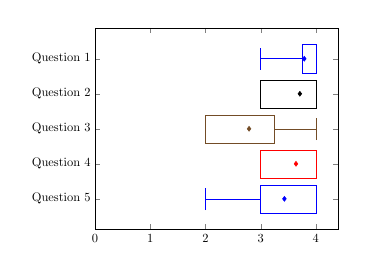
\begin{tikzpicture}[scale=0.45]
  \begin{axis}
    [
    ytick={1,2,3,4,5},
    yticklabels={Question 5, Question 4, Question 3, Question 2, Question 1},
    xmin=0
    ]
    \addplot+[
    boxplot prepared={
      average=3.43,
      upper quartile=4.0,
      lower quartile=3.0,
      upper whisker=4.0,
      lower whisker=2.0
    },
    ] coordinates {};
    \addplot+[
    boxplot prepared={
      average=3.64,
      upper quartile=4.0,
      lower quartile=3.0,
      upper whisker=4.0,
      lower whisker=3.0
    },
    ] coordinates {};
    \addplot+[
    boxplot prepared={
      average=2.79,
      upper quartile=3.25,
      lower quartile=2.0,
      upper whisker=4.0,
      lower whisker=2.0
    },
    ] coordinates {};
    \addplot+[
    boxplot prepared={
      average=3.71,
      upper quartile=4.0,
      lower quartile=3.0,
      upper whisker=4.0,
      lower whisker=3.0
    },
    ] coordinates {};
    \addplot+[
    boxplot prepared={
      average=3.79,
      upper quartile=4,
      lower quartile=3.75,
      upper whisker=4.0,
      lower whisker=3.0
    },
    ] coordinates {};
  \end{axis}
\end{tikzpicture}
\caption{From 14 \system users}
\label{fig:survey1}
\end{subfigure}
~
\begin{subfigure}[t]{0.45\linewidth}
    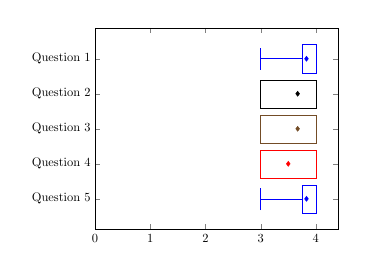
\begin{tikzpicture}[scale=0.45]
  \begin{axis}
    [
    ytick={1,2,3,4,5},
    yticklabels={Question 5, Question 4, Question 3, Question 2, Question 1},
    xmin=0
    ]
    \addplot+[
    boxplot prepared={
      average=3.83,
      upper quartile=4,
      lower quartile=3.75,
      upper whisker=4.0,
      lower whisker=3.0
    },
    ] coordinates {};
    \addplot+[
    boxplot prepared={
      average=3.5,
      upper quartile=4.0,
      lower quartile=3.0,
      upper whisker=4.0,
      lower whisker=3.0
    },
    ] coordinates {};
    \addplot+[
    boxplot prepared={
      average=3.67,
      upper quartile=4.0,
      lower quartile=3.0,
      upper whisker=4.0,
      lower whisker=3.0
    },
    ] coordinates {};
    \addplot+[
    boxplot prepared={
      average=3.67,
      upper quartile=4.0,
      lower quartile=3.0,
      upper whisker=4.0,
      lower whisker=3.0
    },
    ] coordinates {};
    \addplot+[
    boxplot prepared={
      average=3.83,
      upper quartile=4,
      lower quartile=3.75,
      upper whisker=4.0,
      lower whisker=3.0
    },
    ] coordinates {};
  \end{axis}
\end{tikzpicture}
\caption{From 6 \system developers}
\label{fig:survey2}
\end{subfigure}
\caption{Survey results}
 \vspace{-3.0ex} 
\end{figure}

Figure~\ref{fig:survey1} shows the results of the user survey. We can see that most users find \system very useful to locate the root cause. The average score for Question 1 is 3.79, and 11 out of 14 participants find \system very helpful. As for Question 3, \system saves the triage time by 25-50\%. Even in cases that \system cannot correctly locate the root cause, it is still helpful to provide information for further investigation with an average score of 3.43 in Question 5.

For the developer survey, we ask the 6 developers the following 5 questions (Questions 2-5 have the same choices as Question 1):
\begin{itemize}
    \item \textbf{Question 1.} Overall, how convenient is it to change and customize events/rules/domains while using  \system? Answer choices: Convenient(4), Somewhat Convenient(3), Not Convenient(2), Difficult(1).
    \item \textbf{Question 2.} How convenient is it to \emph{change/customize event models} while using \system? 
    \item \textbf{Question 3.} How convenient is it to \emph{add new domains} while using \system? 
    \item \textbf{Question 4.} How convenient is it to \emph{change/customize causality rules} while using \system? 
    \item \textbf{Question 5.} How convenient is it to change/customize \system compared to other SRE tools? 
\end{itemize}

Figure~\ref{fig:survey2} shows the results of the developer survey. Overall, most developers find it convenient to make changes on and customize events/rules/domains in \system. %all questions have very positive responses on average. 5 out of 6 participants find it convenient to make changes on events/rules/domains in \system, while one finds it somewhat convenient. 
% (here domain denotes adding services from different function fields). %We see 3 participants find it somehow convenient in rule customization, indicating that we should make the rule customization easier to use.

\subsection{Lessons learned}
In this section, we share the lessons learned in terms of technology transfer and adoption on using \system in production environments.

\emph{Embedded in Practice.} To build a successful RCA tool in practice, it is important to embed the R\&D efforts in the live environment with SRE experts and users. We have a 30-minute routine meeting daily with an SRE team to manually test and review every site incident. In addition, we actively reach out to the end users for feedback. For example, the users found our initial UI hard to understand. Based on their suggestions, we have introduced alert enrichment with the detailed context of most events, raw metrics, and links to other tools for the next steps. We also make the UI interactive and build user guides, training videos, and sections. As a result, \system has become increasingly practical and well adopted in practice. We believe that R\&D work on observability should be incubated and grown within daily SRE environments. It is also vital to bring developers with rich RCA experience into the R\&D team.

\emph{Vertical Enhancements.} High-confidence and automated vertical enhancements can empower great experiences. \system is enhanced and specialized in critical scenarios such as grouped related %connection stacking 
alerts across services or critical business domain issues, and large-scale scenarios such as infrastructure changes or database issues. Furthermore, the end-to-end automation is also built for integration and efficiency with anomaly detection, RCA, and notification. For notification, domain business anomalies and diagnostic results are sent through communication apps (e.g., slack and email) for better reachability and experience. Within 18 months of R\&D, \system now supports 18 business domains and sub-domains of the company. On average, \system UI supports more than 50 active internal users, and the service sends thousands of results every month. Most of these usages are around the vertical enhancements. 

%\emph{Vertical Enhancement}: During the continued improvements and validations, high accuracy and recurrence scenarios were discovered and enhanced. We created high confidence vertical enhancements that boosted the user's trust and adoption rate. One example here is to use \system for grouped similar connection stacking alerts across the applications or critical domain issues. Thanks to the high customizability of \system, we efficiently enhanced the vertical experiences, such as fine-tuning and specialized events. We then created an end-to-end flow that includes detection, RCA, and notification. Lots of essential incidents with complicated context were supported, such as infra change and database issues. Then, overall efficiency is improved through integrations with other critical site tools. We also attach diagnostic results in the communication apps (e.g., slack, email, and ServiceNow) for better visibility and reachability. Within 18 months of R\&D, we have hundreds of users per month access to the application for 18 domains and sub-domains RCA. We believe for any AIOPs product like \system - vertical enhancements which focus on the domain use cases are essential to success. 


\emph{Data and Tool Reliability.} Reliability is critical to \system itself and requires a lot of attention and effort. For example, if a critical event is missing, \system may infer a totally different root cause, which would mislead users. %the whole causality of an incident may be affected. In this case, it is not helpful that the user can assume only the related metrics/status are fine. 
We estimate the alert accuracy 
%($f1$) 
to be greater than 0.6 in order to be useful. Recall is even more important since \system can effectively eliminate false positive alerts based on the casual ranking. Since there are hundreds of different metrics supported in \system, we spend time to ensure a robust back end by adding partial and dynamic retry logic and high-efficiency cache. \system's unsuccessful cases can be caused by imperfect data, flawed algorithms, or simply code defects. To better trace the reason behind each unsuccessful case, we add a tracing component. Every \system request can be traced back to atomic actions such as retrieving data, data cleaning, and anomaly detection via algorithms.

\emph{Trade-off among Models.} The accuracy and scalability trade-off among anomaly detection models should be carefully considered and tested. In general, some algorithms such as deep-learning-based or ensemble models are more adaptive and accurate than typical ones such as traditional ML or statistical models. However, the former requires more computation resources, operational efforts, and additional system complexities such as training or model fine-tuning. Due to the actual complexities and fast-evolving nature of our context, it is not possible to scale each model (e.g., deep-learning-based models), nor have it deeply customized for every metric at every level. Therefore, while selecting models, we must make careful trade-off in aspects such as accuracy, scalability, efficiency, effort, and robustness. In general, we first set different ``acceptance'' levels by analyzing each event's impact and frequency, and then test different models in staging and pick the one that is good enough. For example, a few alerts such as ``high thread usage'' are defined by thresholds and work just fine even without a model. Some alerts such as  ``service client error'' are more stochastic and require coverage on every metric of every service, and thus we select fast and robust statistical models and actively conduct detection on the fly.  %Business and domain anomaly events can trigger our triaging flow and diagnostics automatically. SRE and monitoring teams spend more time for better and accurate results, such as exercising deep learning approaches, manually correlate critical signals and active improvements for the false positives.

\emph{Phased Incorporation of ML.} In the current industrial settings, ML-powered RCA products still require effective knowledge engineering. Due to the higher complexity and lower ``signal to noise ratio'' of real production incidents, many existing approaches cannot be applied in practice. We believe that the knowledge engineering capabilities can facilitate adoption of technologies such as AIOps. Therefore, \system is designed to be highly customizable and easy to infuse SRE knowledge and to achieve high effectiveness and efficiency. Moreover, a multi-scenario RCA tool requires various and interpretable events from different detection strategies. Auto-ML-based anomaly detection or unsupervised RCA for large service ecosystems is not yet ready in such context.
% resulting in that taking a general ML model is currently not practical in industrial settings.
As for the path of supervised learning, the training data is tricky to label and vulnerable to potential cognitive bias. 
% from SRE engineers
Lastly, the end users often require complete understanding to fully adopt new solutions, because there is no guarantee of correctness. Many recent ML algorithms (e.g., ensemble and deep learning) lack interpretability. Via the knowledge engineering and graph capabilities, \system is able to explain diversity and causality between ML-model-driven and other types of events. Moving forward, we are building a white-box deep learning approach with causal graph algorithms where the causal link weights are parameters and derivable. 
%, while some are manually tuned or detected by rules for certainty and interpretability. For root cause analysis in practice, taking diversified predictive ML anomalies as the major inputs into another ML layer for  root cause analysis, seems too ideal and difficult as mentioned in Section~\ref{sec:intro}. Additionally, there is also a ``chicken-and-egg'' issue for the supervised learning path: collecting training datasets first can be risky and is hard to happen in the SRE domain. Via a graph-based approach, \system is able to explain how diversified and low-level ML events and their connectivity. Also, it effectively and efficiently solve most of the challenge. Lastly, we are more ready for other intelligent solutions with the dataset of 1000+ real production incidents for training, and our AIOPs infrastructure.

%\section{Discussion}

In this section, we discuss some future extension or improvements on the system. 

As we discussed in Section~\ref{sec:anomalyrelated}, there are many related works for anomaly detection. Some approaches are using adaptive concept drifting, which can self-adapt to the target event without manual tuning~\cite{ma2018robust}. One major burden in our event construction is that we need to build different detection strategies/algorithms for different events, while some events are still needed to be manually tuned or detected by rules. Auto-ML is yet to come for anomaly detection, and the interpretability of the result is also a big challenge for end-to-end usability. The filter range for some events also needs manual tuning which requires large amount of domain expertise and is not robust. As of now, we are investing self-adaptive approaches and building time series metrics anomaly detection platform to reduce the event on-boarding cost. 

Also, our approach, which requires a fair amount of ``one-time" effort, utilizes rules to build links between events. A lot of the rules have similar patterns. Despite that our users prefer to have their own control, rules can be inferred from historical patterns. A great extension to this work is the use of machine learning or grammar inference techniques~\cite{wu2019reinam} to automatically or semi-automatically infer the rules.

%At last, since the framework is robust and generic to many use cases, we are planning to release it as open-source system so that we can allow different kinds of users to customize the system based on their own dependencies/events/domains. This also gives us the chance to further speculate \system's performance under different customized scenarios. 


\section{Summary}

We performed a series of galactic disk $N$-body simulations
to investigate the formation and dynamical evolution of spiral arm 
and bar structures in stellar disks which are embedded in live 
dark matter halos.
We adopted a range of initial conditions where the models have similar halo 
rotation curves, but different masses for the disk and bulge components, 
scale lengths, initial $Q$ values, and halo spin parameters.
The results indicate that the bar formation epoch increases exponentially 
as a function of the disk mass fraction with respect to the total mass at the 
reference radius (2.2 times the disk scale length), $f_{\rm d}$.
This relation is a consequence of swing amplification~\citep{1981seng.proc..111T},
which describes the amplification rate of the spiral arm when it transitions from 
leading arm to trailing arm because of the disk's differential rotation.
Swing amplification depends on the properties that characterize the disk, 
Toomre's $Q$, $X$, and $\Gamma$. The growth rate reaches its maximum
for $1<X<2$,  although the position of the peak slightly depends on $Q$ as well as on
$\Gamma$. We computed $X$ for 
$m=2$ ($X_2$), which corresponds to a bar or two-armed spiral, 
for each of our models and found that this value is related to the bar's
formation epoch.

The bar amplitude grows most efficiently when $1<X_2<2$. For models 
with $1<X_2<2$ the bar develops immediately after the start 
of the simulation. As $X_2$ increases beyond $X_2=2$, the growth rate
decreases exponentially. We find that the bar formation epoch increases
exponentially as $X_2$ increases beyond $X_2=2$, in other words
$f_{\rm d}$ decreases. The bar formation epoch exceeds a Hubble time
for $f_{\rm d}\lesssim 0.35$.

Apart from $X$, the growth rate is also influenced by $Q$ where
a larger $Q$ results in a slower growth. This indicates that the bar formation
occurs later for larger values of $Q$. 
Our simulations confirmed this and showed that for the bar ($m=2$) the growth rate
is predicted by swing amplification and becomes visible when it grows beyond a certain amplitude.

Toomre's swing amplification theory further predicts that
the number of spiral arms is related to the mass of the disk, with
massive disks having fewer spiral arms. In addition, larger $\Gamma$
predicts a smaller number of spiral arms.
We confirmed these relations in our simulations. 
The shear rate ($\Gamma$) also affects the pitch angle of spiral
  arms. We further confirmed that our result is consistent with previous
studies.

We found that the disk-to-total mass fraction ($f_{\rm d}$)
and the shear rate ($\Gamma$) are the most important parameters that determine the
morphology of disk galaxies. 
When juxtaposing our models with the Hubble sequence,
the fundamental subdivisions of (barred-)spiral galaxies with 
massive bulges and tightly wound-up spiral arms from S(B)a to S(B)c is 
also be observed as a sequence in our simulations. Where the models 
with either massive bulges or massive disks have more tightly
wound spiral arms. This is because having both a massive disk and bulge results in 
a larger $\Gamma$, i.e., more tightly wound spiral arms. 


Once the
bar is formed it starts to heat the outer parts of the disk.
From this point onwards, 
the self-gravitating spiral arms disappear.
This may be in part caused by the 
lack of gas in our simulations. 
After the bar grows, we no longer discern  
spiral arms in the outer regions of the disk. This could imply
that gas cooling and star formation are required in order to 
maintain spiral structures in barred spiral galaxies for over 
a Hubble time~\citep{1981ApJ...247...77S,1984ApJ...282...61S}.


Our simulations further indicate that non-barred grand-design spirals are
transient structures which immediately evolve into barred
galaxies. Swing amplification teaches us that a massive disk is
required to form two-armed spiral galaxies. This condition, at the
same time, satisfies the short formation time of the bar structure.
Non-barred grand-design spiral galaxies therefore must evolve into barred
galaxies.  We consider that isolated non-barred grand-design spiral galaxies 
are in the process of developing a bar.





\bibliographystyle{IEEEtran}
\bibliography{references}


\end{document}

